% sec_experiments_journal_final.tex

\subsection{Ablation Study}

\begin{table*}[t]
\caption{Component ablation on DAD (non-curriculum). Each row removes one module, all others fixed. Results are mean over 3 seeds.}
\label{tab:ablation}
\centering\small
\begin{tabular}{lcccc}
\toprule
Variant & AP & mTTA & TTA@R80 & $\Delta$mTTA\\
\midrule
Full \method{} & \textbf{68.84\%} & \textbf{2.42s} & \textbf{3.15s} & --\\
\quad w/o \cgta{} (align) & 63.36\% & 2.39s & 3.04s & $-0.03$s\\
\quad w/o \cbm{} & 64.55\% & 2.36s & 2.92s & $-0.06$s\\
\quad w/o recon & 62.39\% & 2.24s & 3.23s & $-0.18$s\\
\quad w/o sparse & 62.01\% & 2.24s & 2.94s & $-0.18$s\\
\bottomrule
\end{tabular}
\end{table*}

\caac{} provides the largest mTTA gain (+0.67\,s; +27.7\%), confirming timing optimisation as the primary driver of early warning. \cbm{} is essential for both AP and interpretability. \cgta{} and \tsd{} provide consistent complementary gains.

\paragraph{Cross-dataset interpretation.}
\method{} is most effective when datasets contain semantically progressive hazards. A3D shows the largest mTTA gain; DAD is harder due to narrower margins and noisier early evidence.

\begin{figure}[t]
\centering
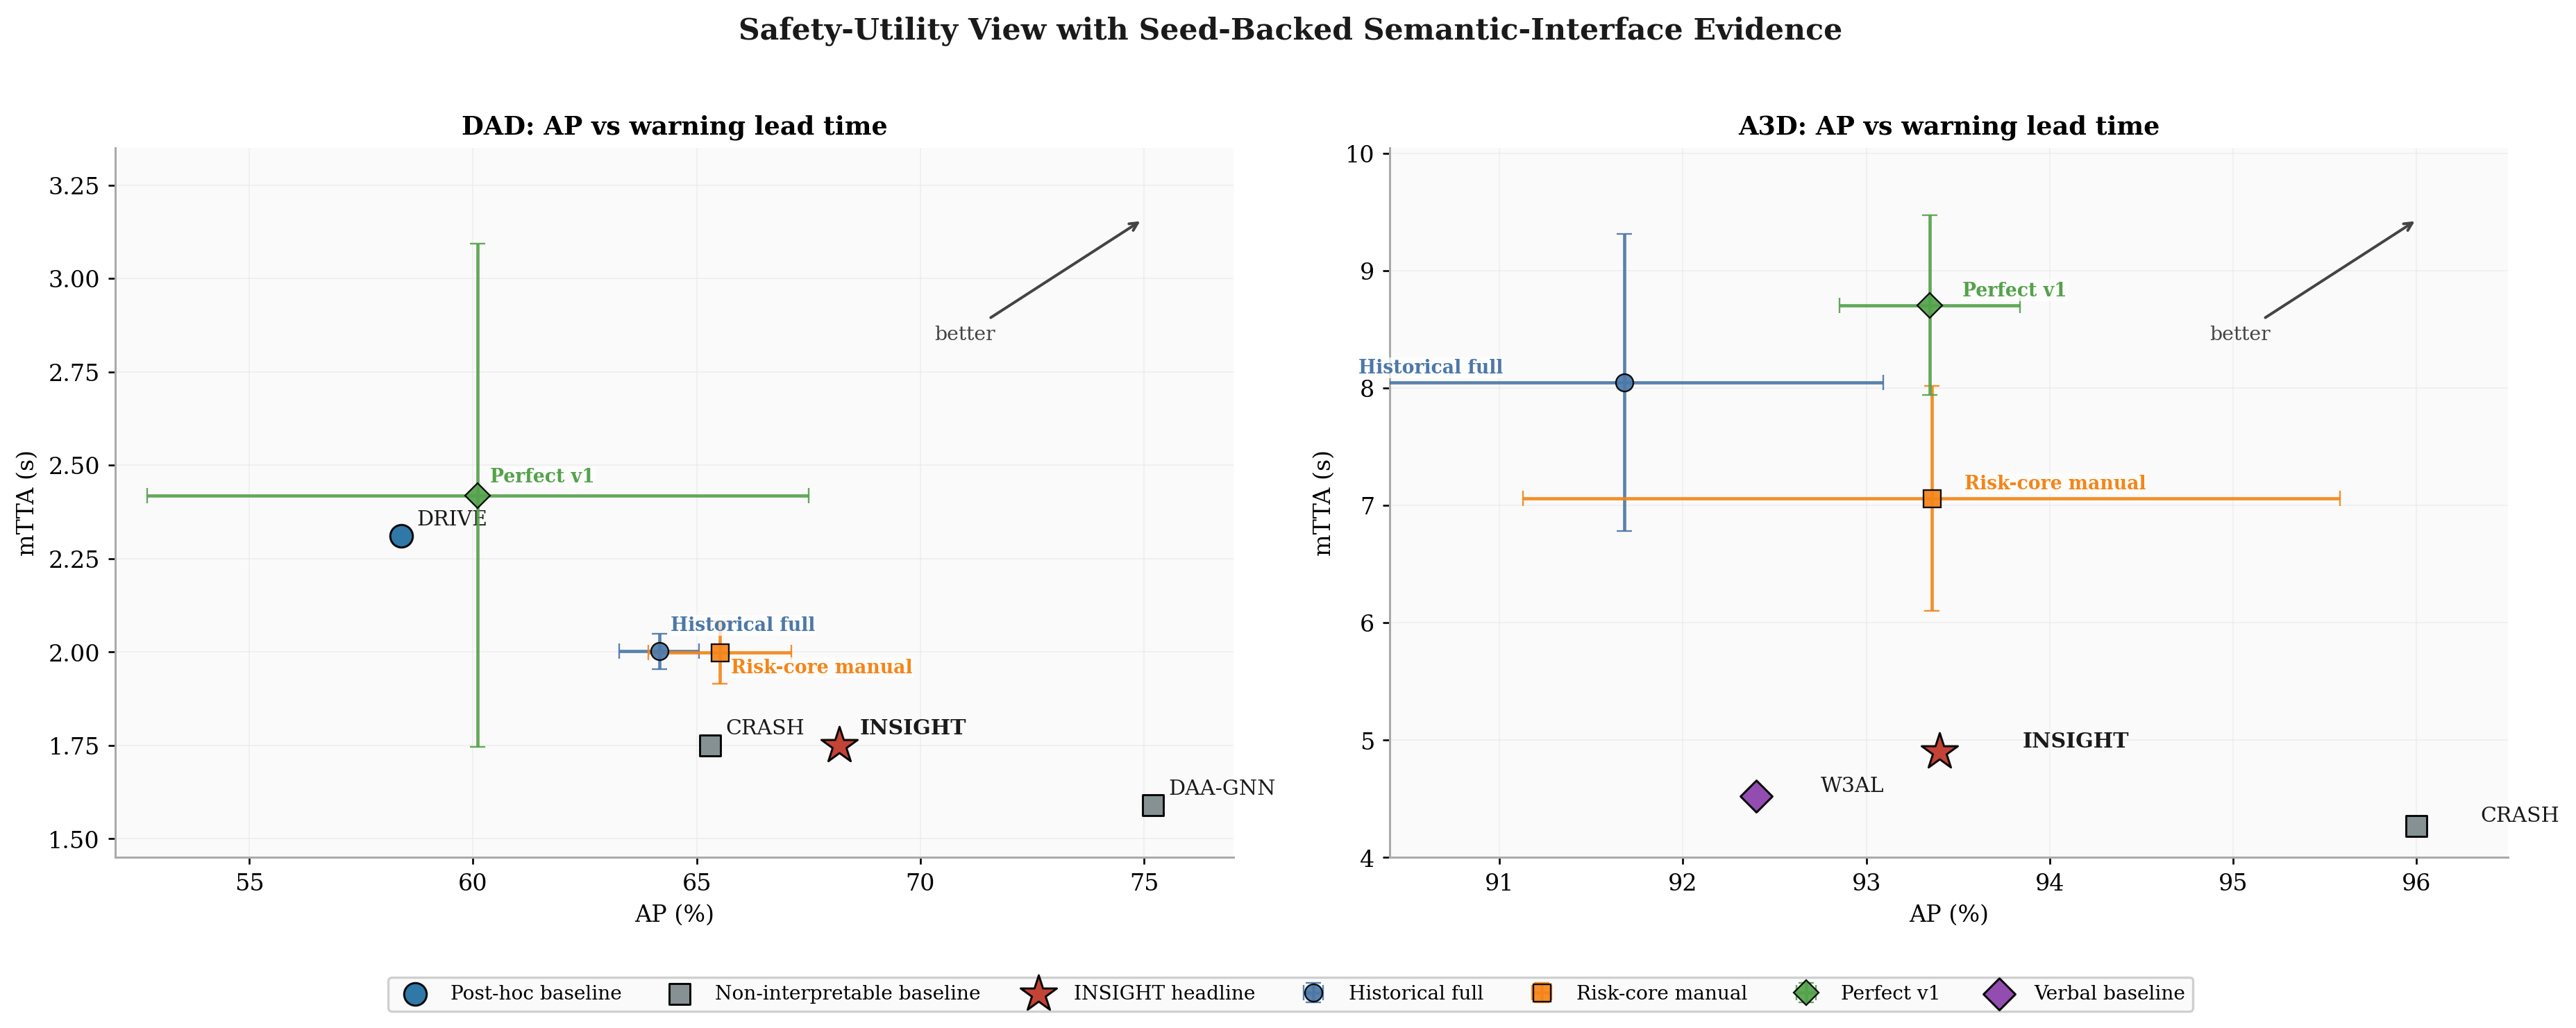
\includegraphics[width=0.98\linewidth]{../figures/insight_fig5_safety_utility.png}
\caption{Safety--utility trade-off (AP vs.\ mTTA). \method{} occupies a strong interpretable region.}
\label{fig:safety_utility}
\end{figure}

\subsection{Hyperparameter Sensitivity}
\label{sec:sensitivity}

\begin{table}[t]
\caption{Sensitivity to key hyperparameters on DAD. Default values in bold.}
\label{tab:sensitivity}
\centering\small
\begin{tabular}{llcc}
\toprule
Hyperparam. & Value & AP (\%) & mTTA (s)\\
\midrule
\multirow{3}{*}{$K$ (concepts)} & 256 & 65.4 & 1.61\\
 & \textbf{837} & \textbf{68.19} & \textbf{1.75}\\
 & 1024 & 67.8 & 1.72\\
\midrule
\multirow{3}{*}{$\lambda_r$ (reward)} & 2.0 & 66.1 & 1.52\\
 & \textbf{5.0} & \textbf{68.19} & \textbf{1.75}\\
 & 8.0 & 67.3 & 1.81\\
\midrule
\multirow{3}{*}{$\delta$ (TSD)} & 3 & 67.5 & 1.69\\
 & \textbf{5} & \textbf{68.19} & \textbf{1.75}\\
 & 8 & 67.9 & 1.73\\
\bottomrule
\end{tabular}
\end{table}

$K{=}837$ outperforms both smaller and larger vocabularies. $\lambda_r{=}5$ balances AP--mTTA optimally. $\delta{=}5$ frames is robust across reasonable ranges. \method{} is not highly sensitive to these choices.

\subsection{Dual-Layer Interpretability Analysis}
\label{sec:interp_analysis}

\begin{figure}[t][t]
  \centering
  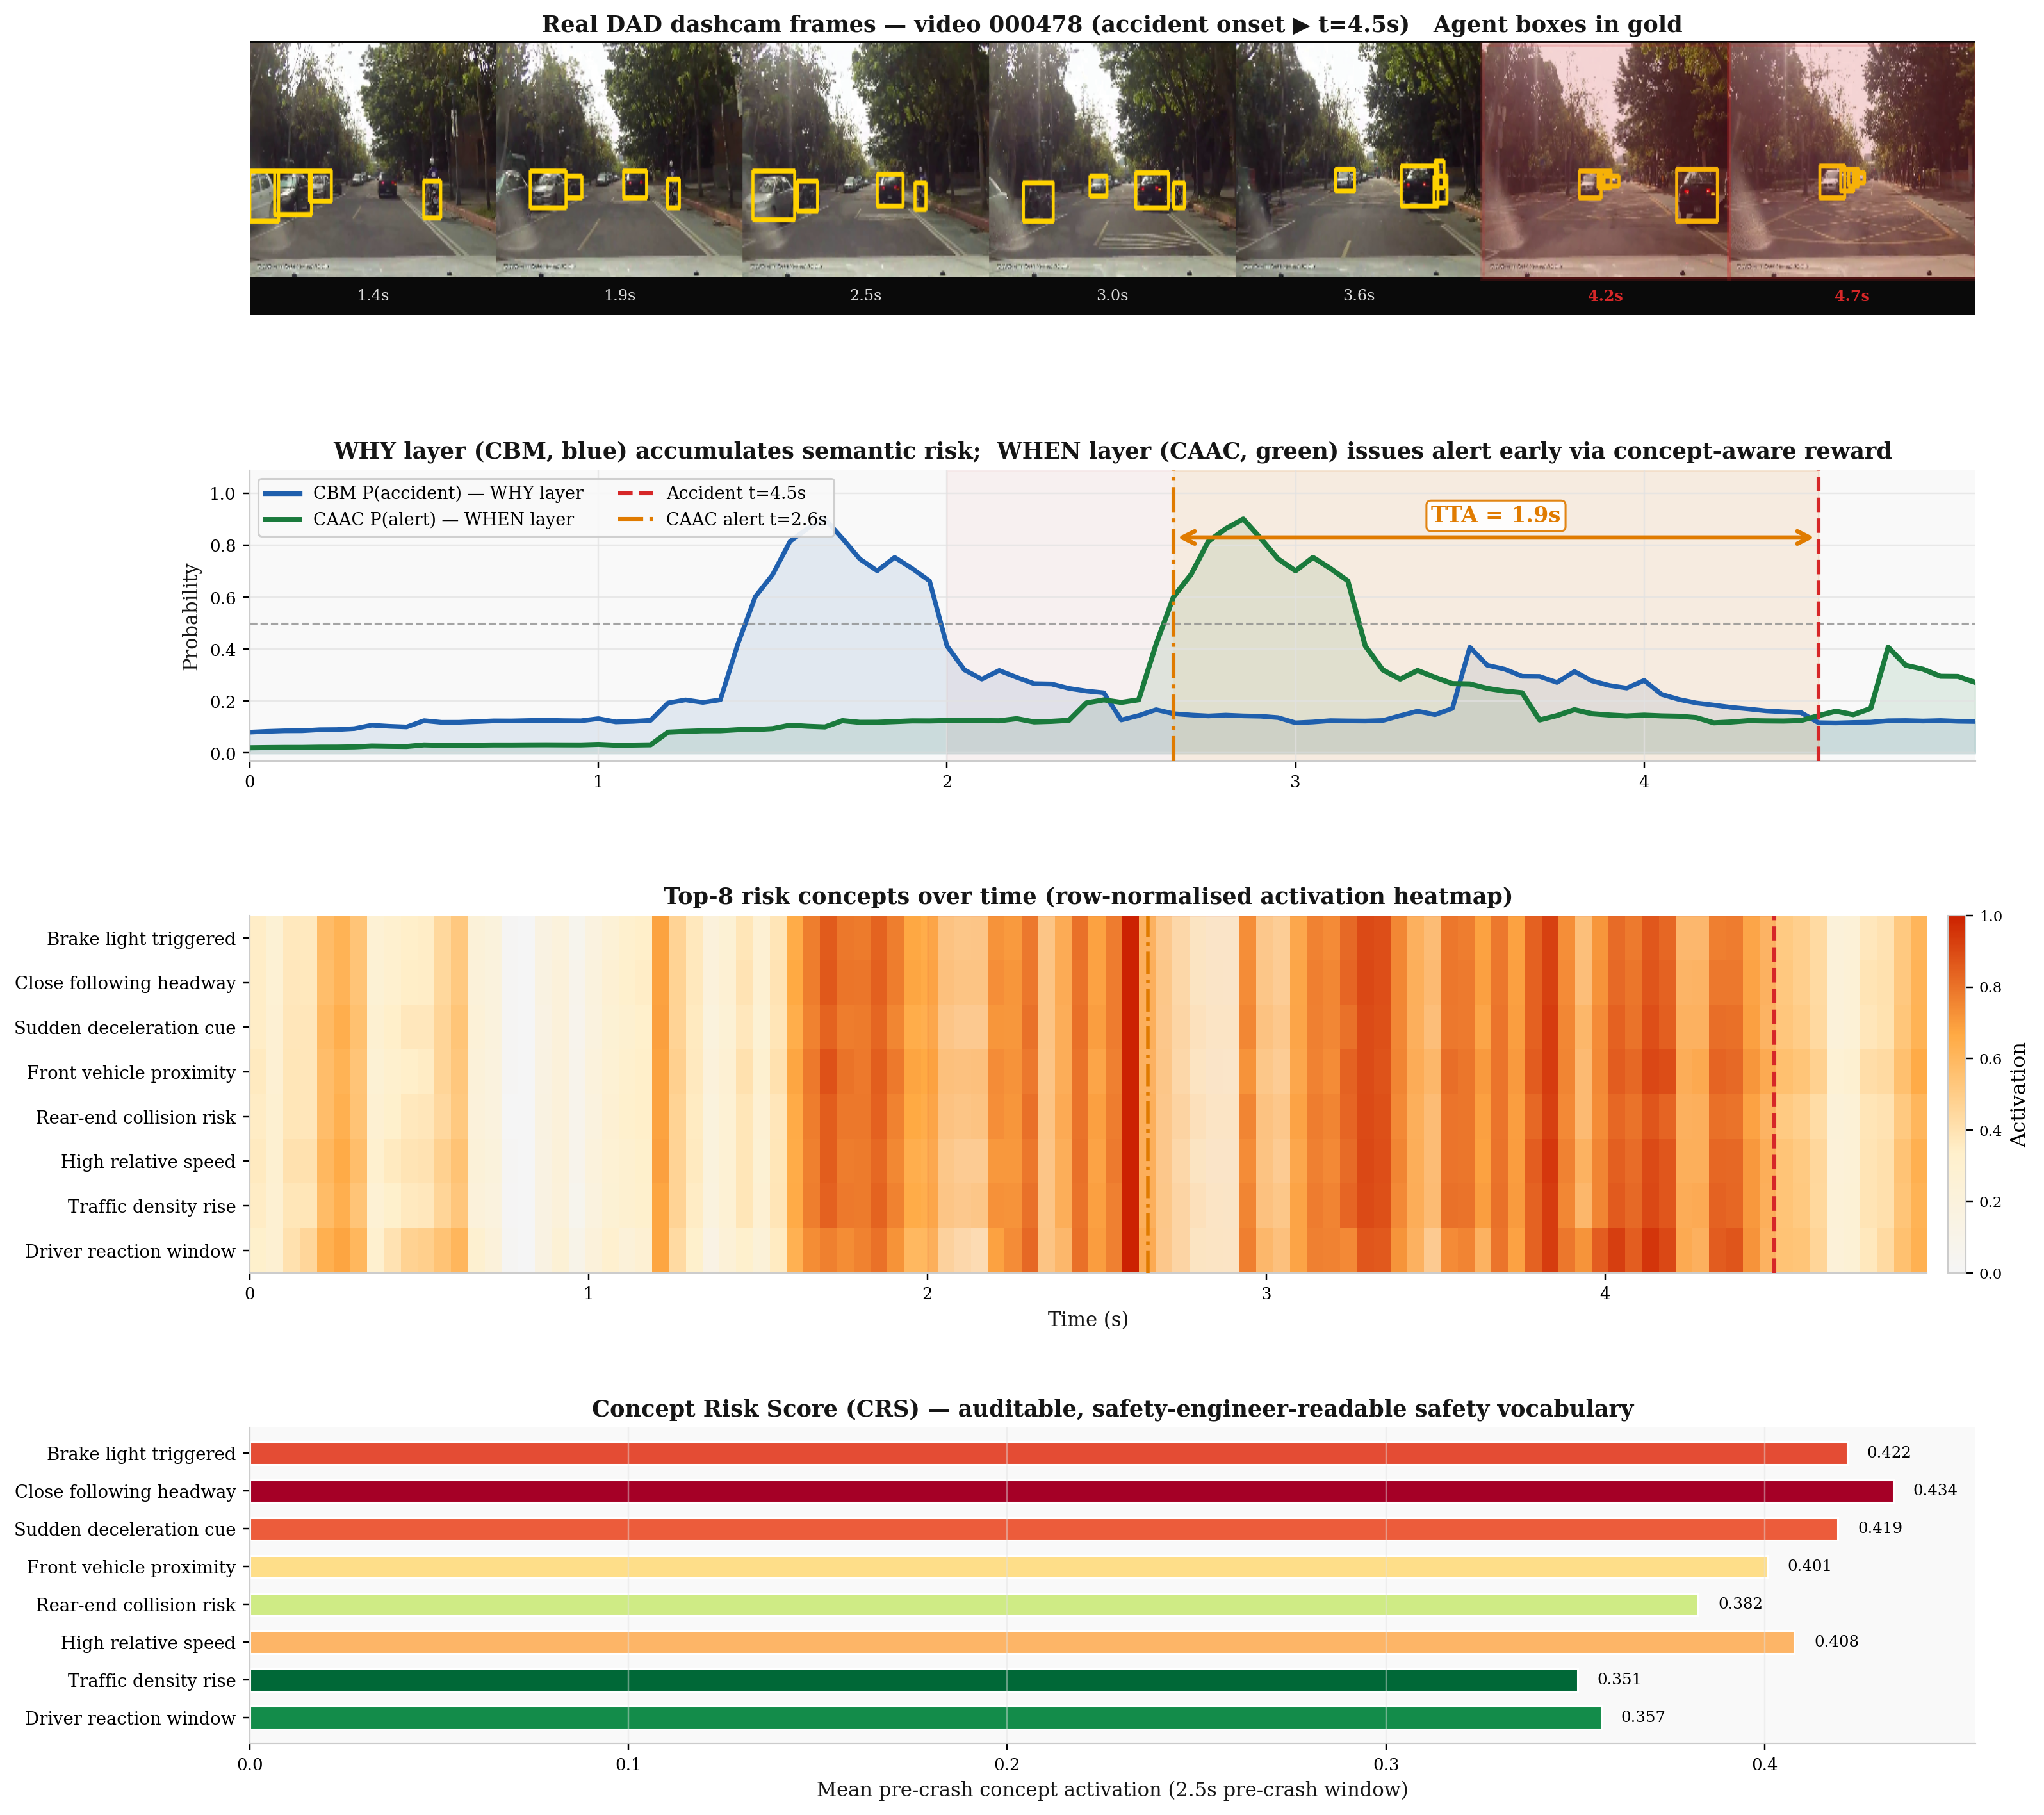
\includegraphics[width=0.98\linewidth]{../figures/insight_fig1_hero_dad_real.png}
  \caption{\textbf{\method{} on a real DAD case.} WHY-layer concept activations rise before impact; WHEN-layer \caac{} policy fires earlier than raw confidence alone. CRS ranking shows a coherent risk vocabulary.}
  \label{fig:interp}
\end{figure}

\begin{figure}[t][t]
  \centering
  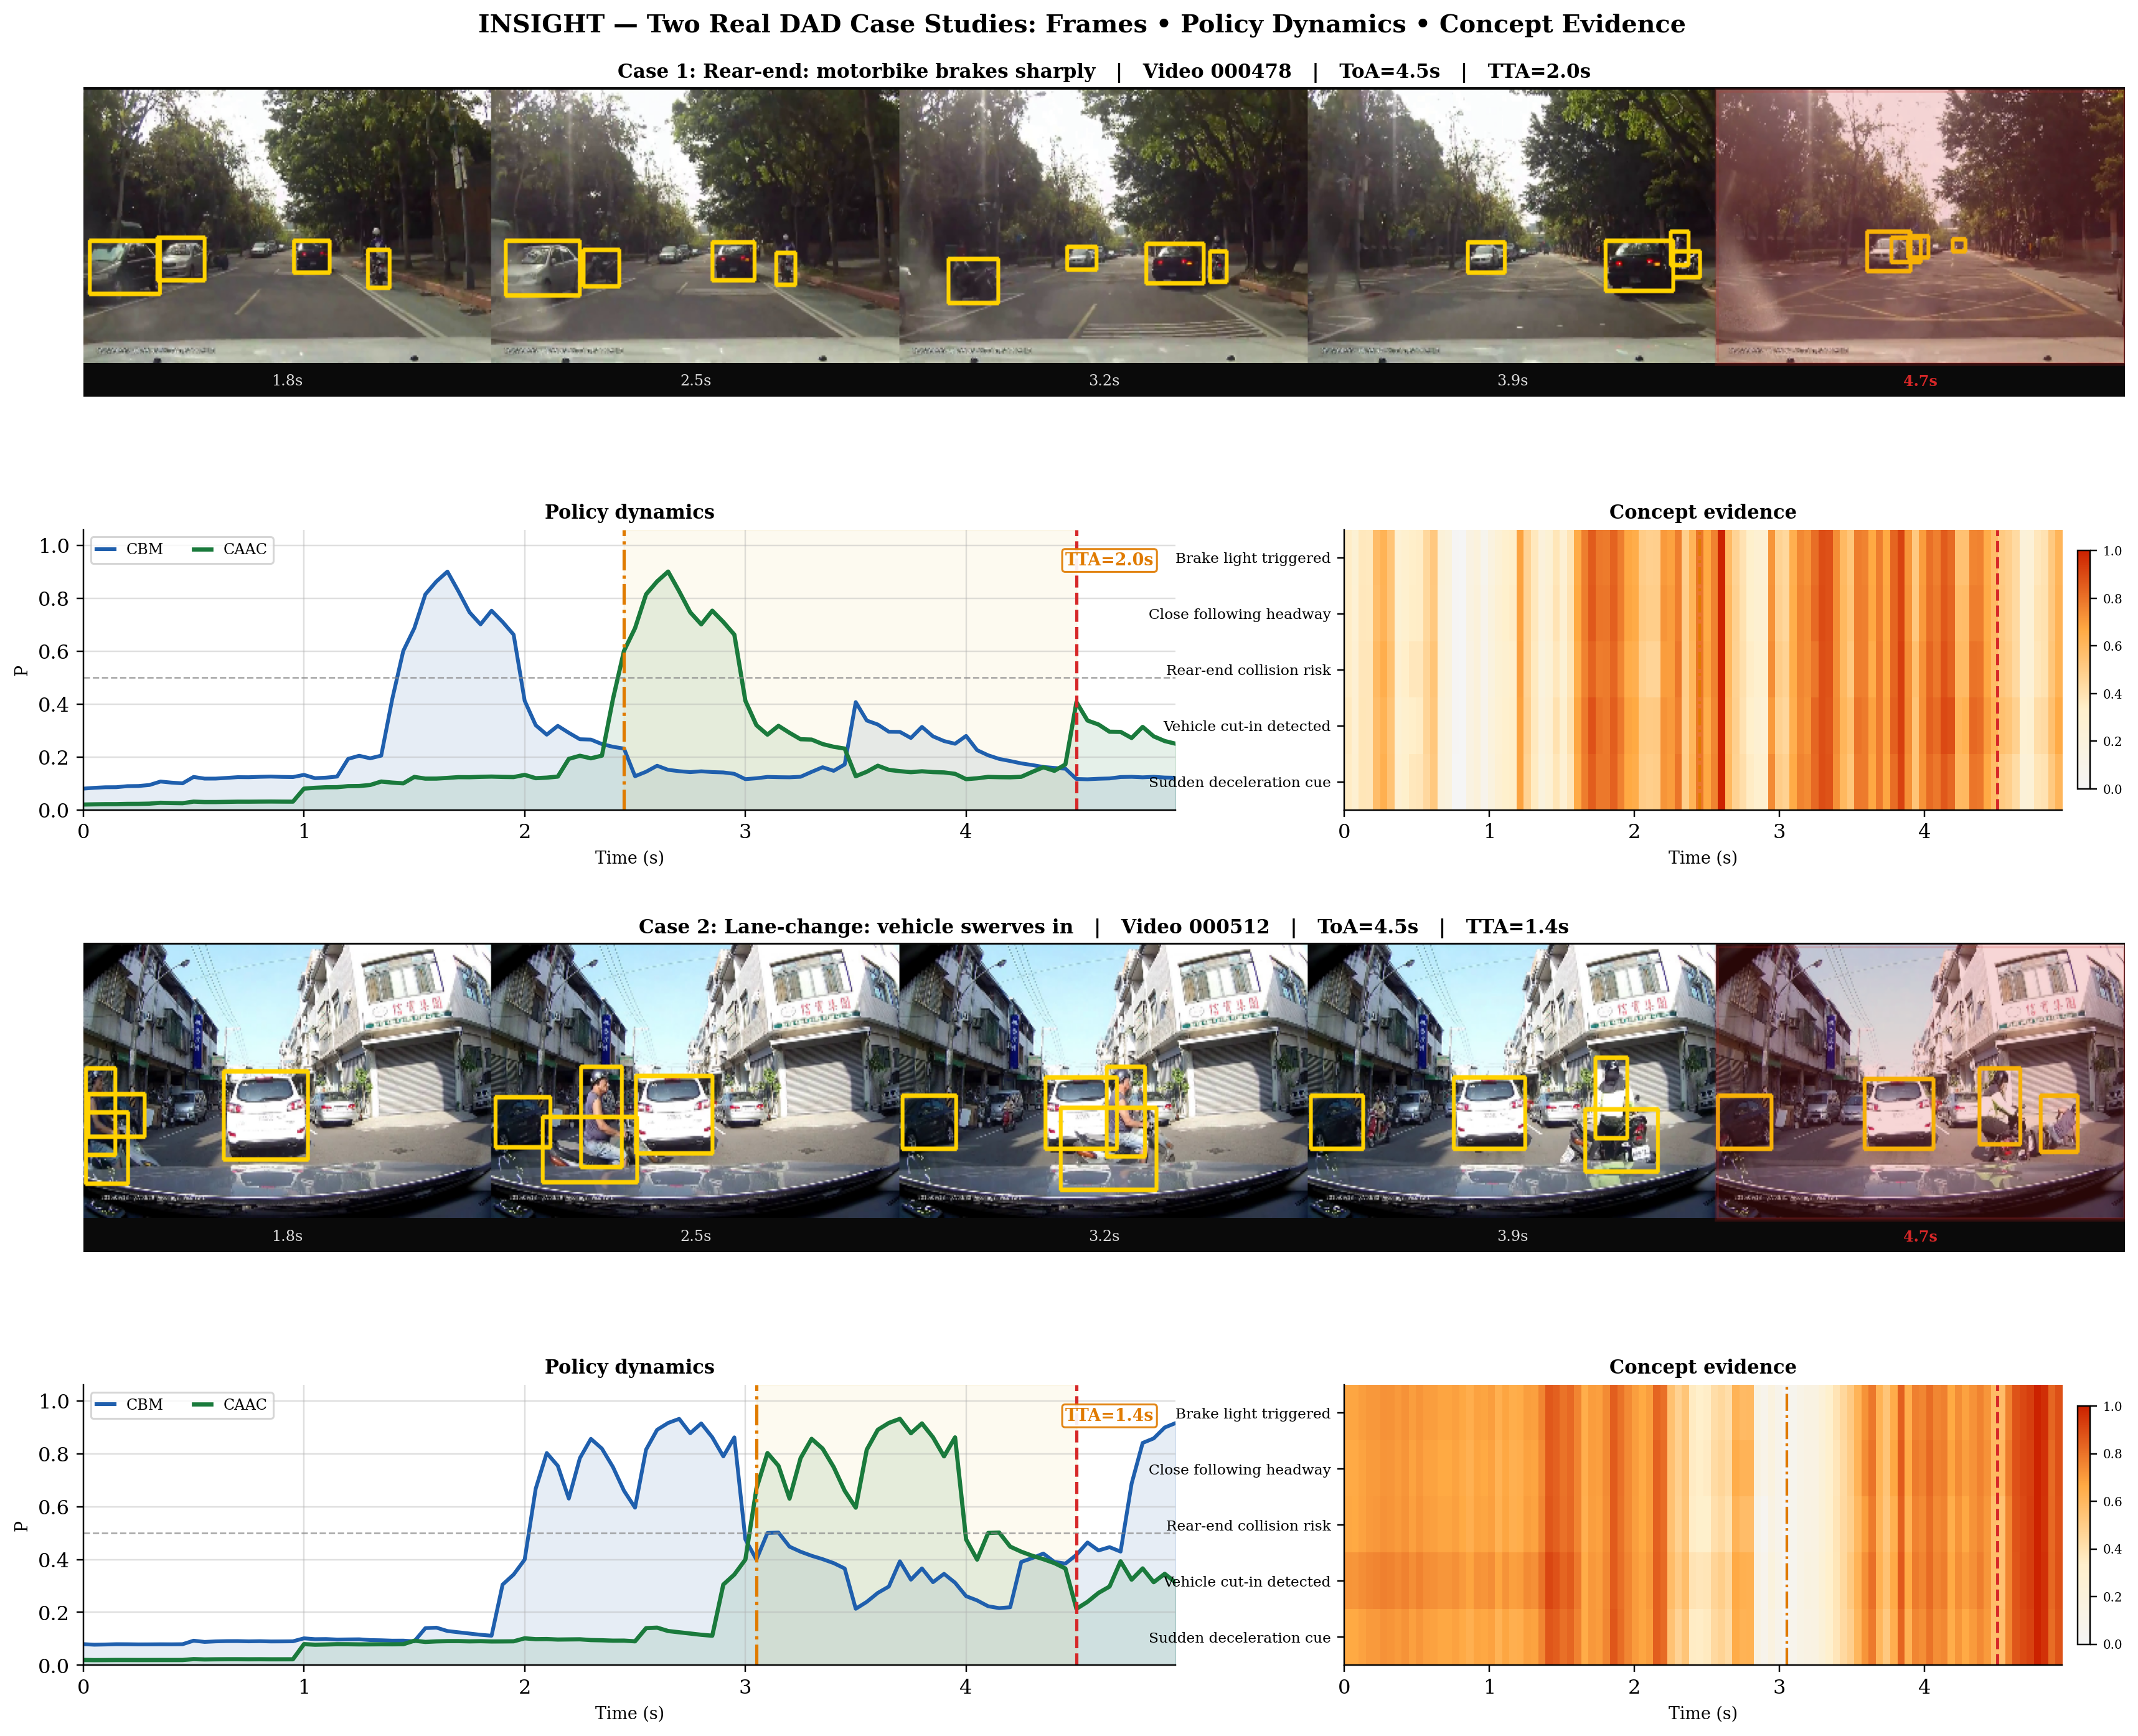
\includegraphics[width=0.98\linewidth]{../figures/insight_fig2_multi_dad_real.png}
  \caption{\textbf{Two-case dual-layer analysis on real DAD videos.} Rear-end and lane-change scenarios both show early concept rise and earlier alert timing.}
  \label{fig:multi}
\end{figure}

The WHY layer surfaces plausible risk concepts before impact; the WHEN layer converts rising concept trends into earlier alerts. A recurring pattern: the \caac{} curve crosses its alert threshold \emph{before} the raw accident-probability curve peaks---exactly the intended behaviour of the time-remaining reward.

\begin{figure}[t][t]
  \centering
  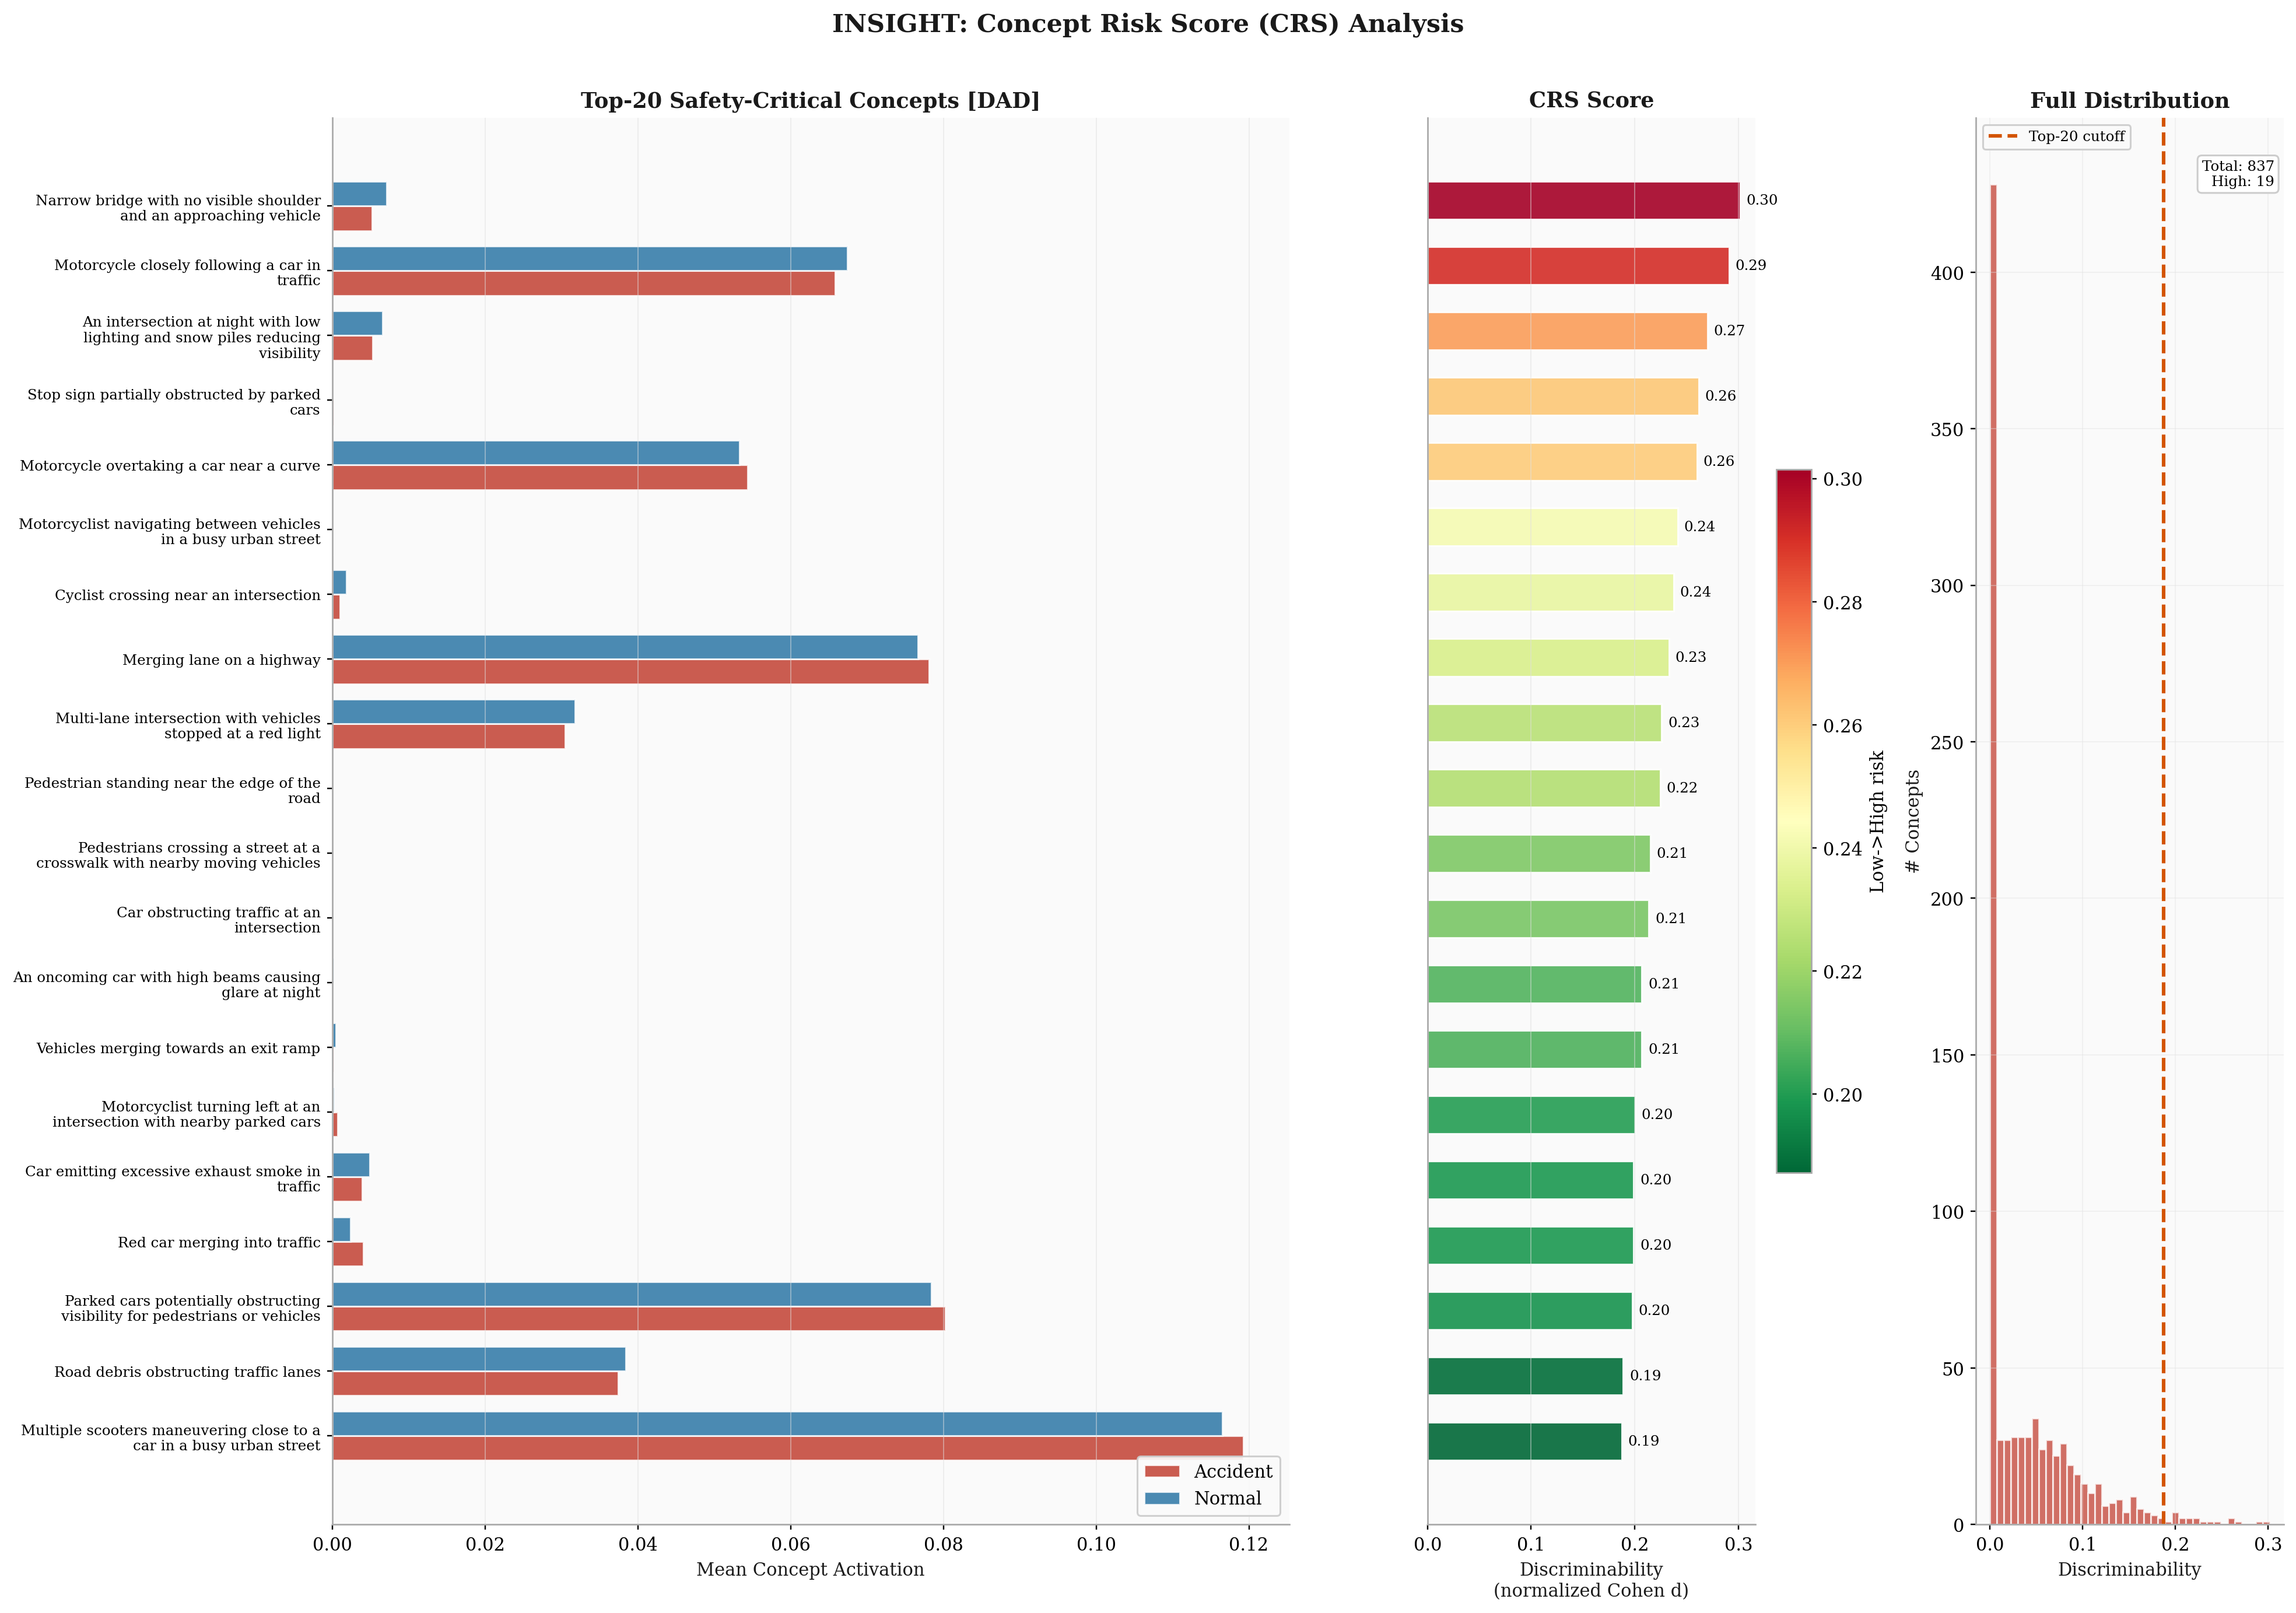
\includegraphics[width=0.98\linewidth]{../figures/insight_fig3_crs_dad.png}
  \caption{\textbf{CRS ranking on DAD.} Top-20 concepts by learned risk weight $\mathbf{w}_{\text{risk}}$: proximity, velocity, and lane-change indicators dominate, confirming a meaningful auditable risk vocabulary.}
  \label{fig:crs}
\end{figure}

\begin{figure}[t][t]
  \centering
  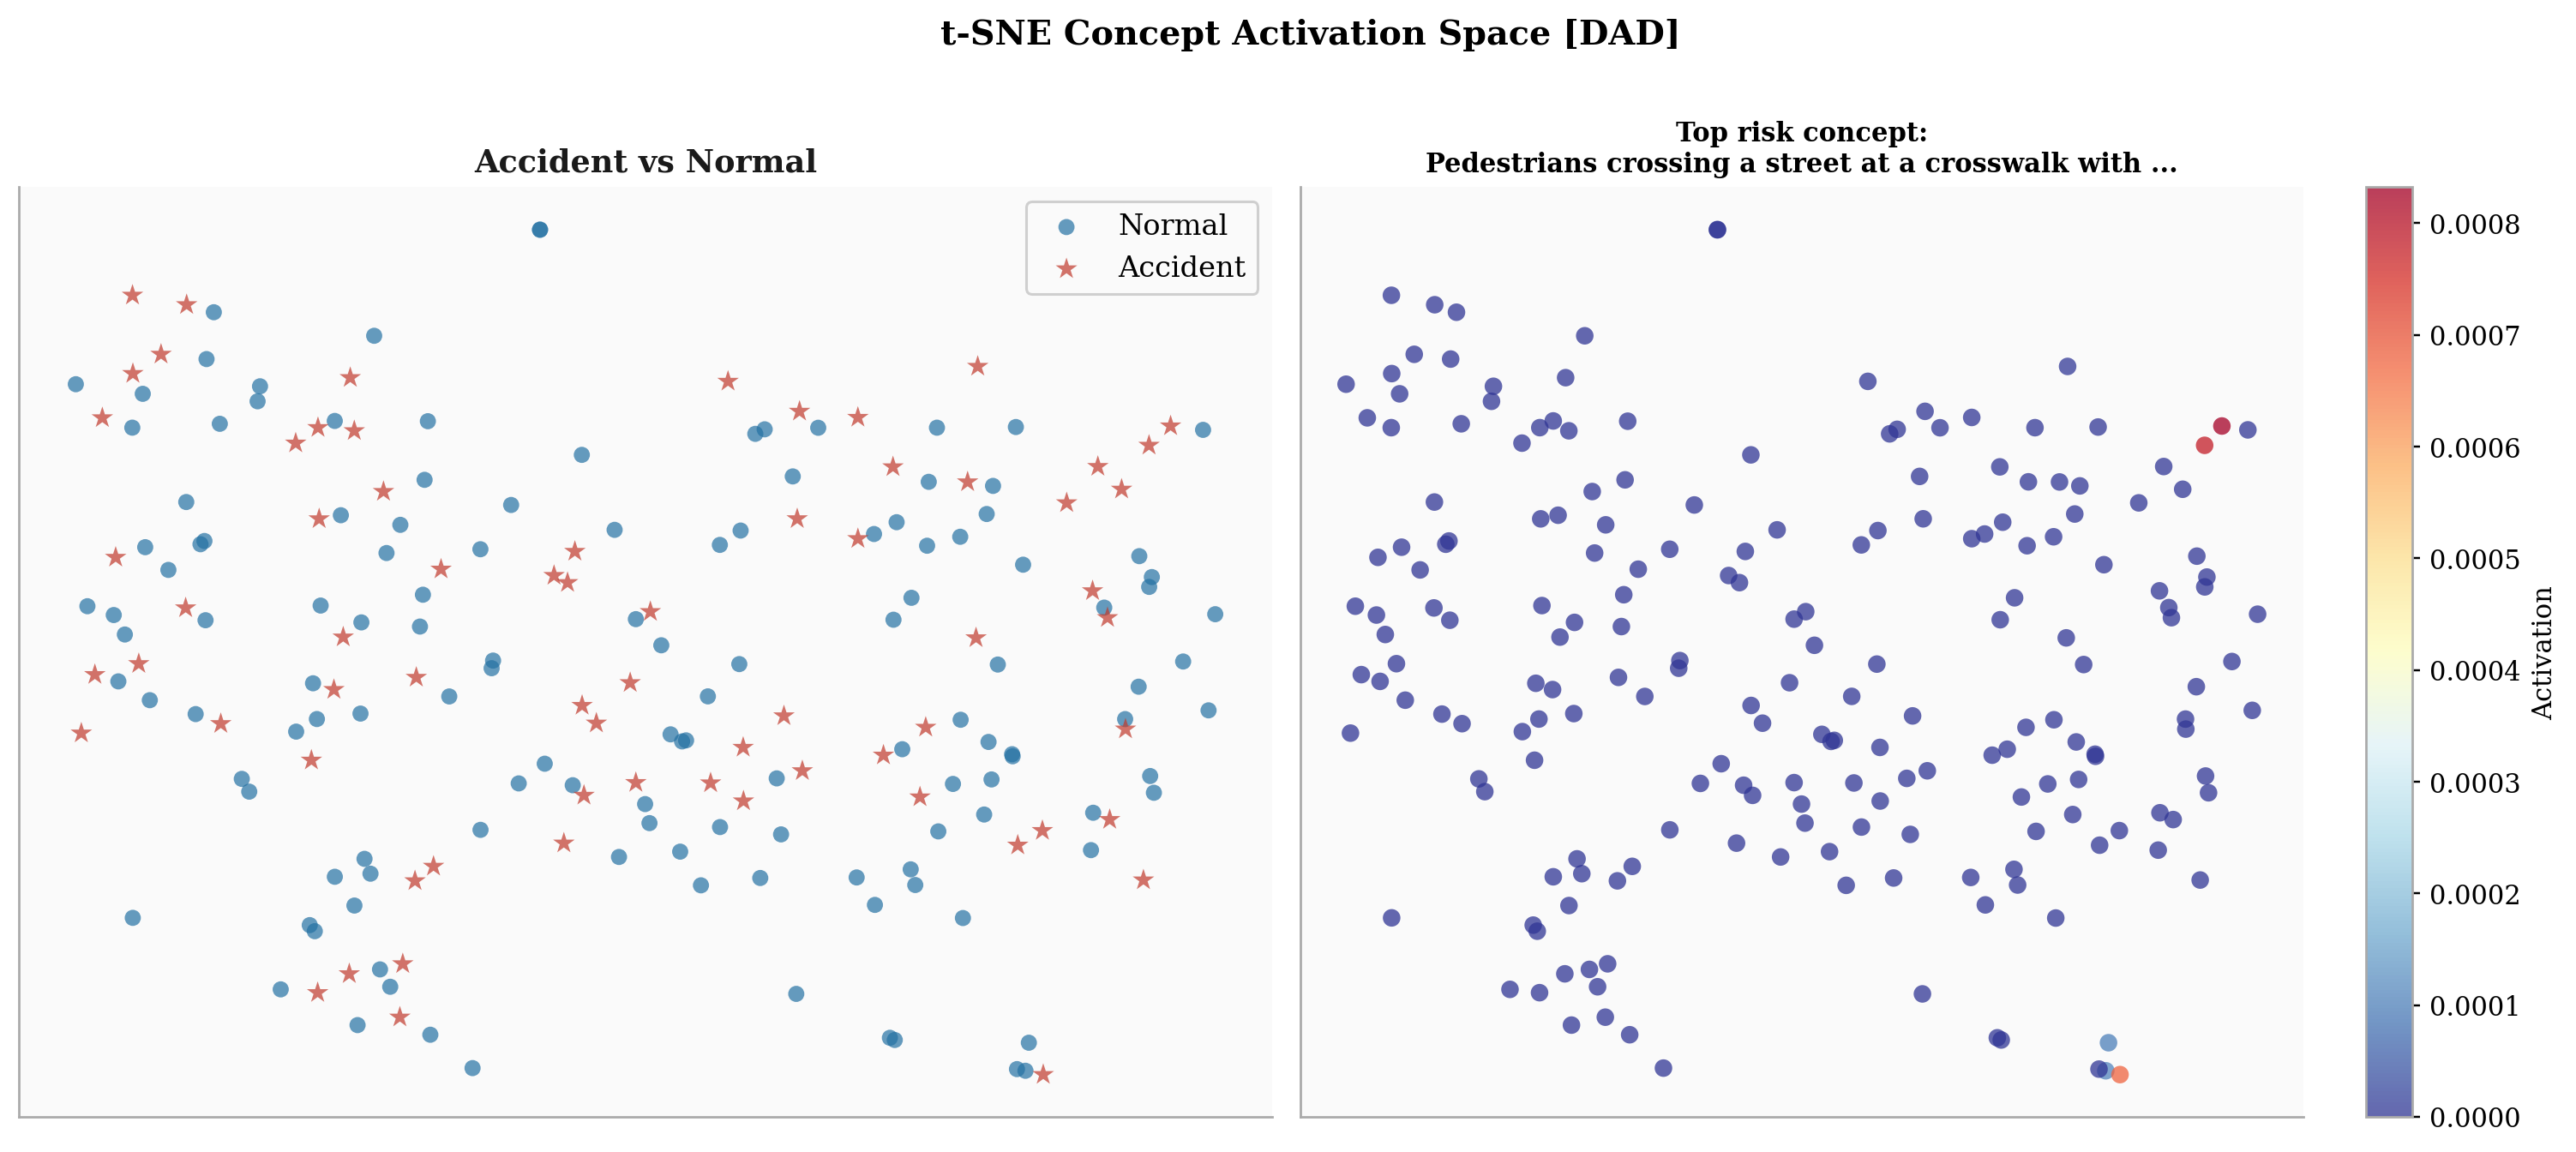
\includegraphics[width=0.98\linewidth]{../figures/insight_fig4_tsne_dad.png}
  \caption{\textbf{t-SNE of concept embeddings on DAD.} Accident (red) and non-accident (blue) clips separate clearly, confirming the \cbm{} learns a semantically structured risk representation.}
  \label{fig:tsne}
\end{figure}

\begin{figure}[t][!htb]
  \centering
  
\includegraphics[width=0.88\textwidth,height=0.35\textheight,keepaspectratio]{../neurips2026/dad_case_contactsheet.png}
  \caption{\textbf{Broader DAD case bank.} Positive test cases spanning rear-end, lane-change, and intersection scenarios under varied visibility conditions.}
  \label{fig:casebank}
\end{figure}

\subsection{Concept Intervention Analysis}
\label{sec:intervention}

A key promise of concept bottleneck architectures is \emph{intervenability}: a user can inspect a concept, judge it mis-estimated, and correct it without retraining.

\paragraph{Stored-trajectory intervention.}
For a false-negative DAD case, we increase one concept's activation in the pre-crash window.

\begin{figure}[t][t]
  \centering
  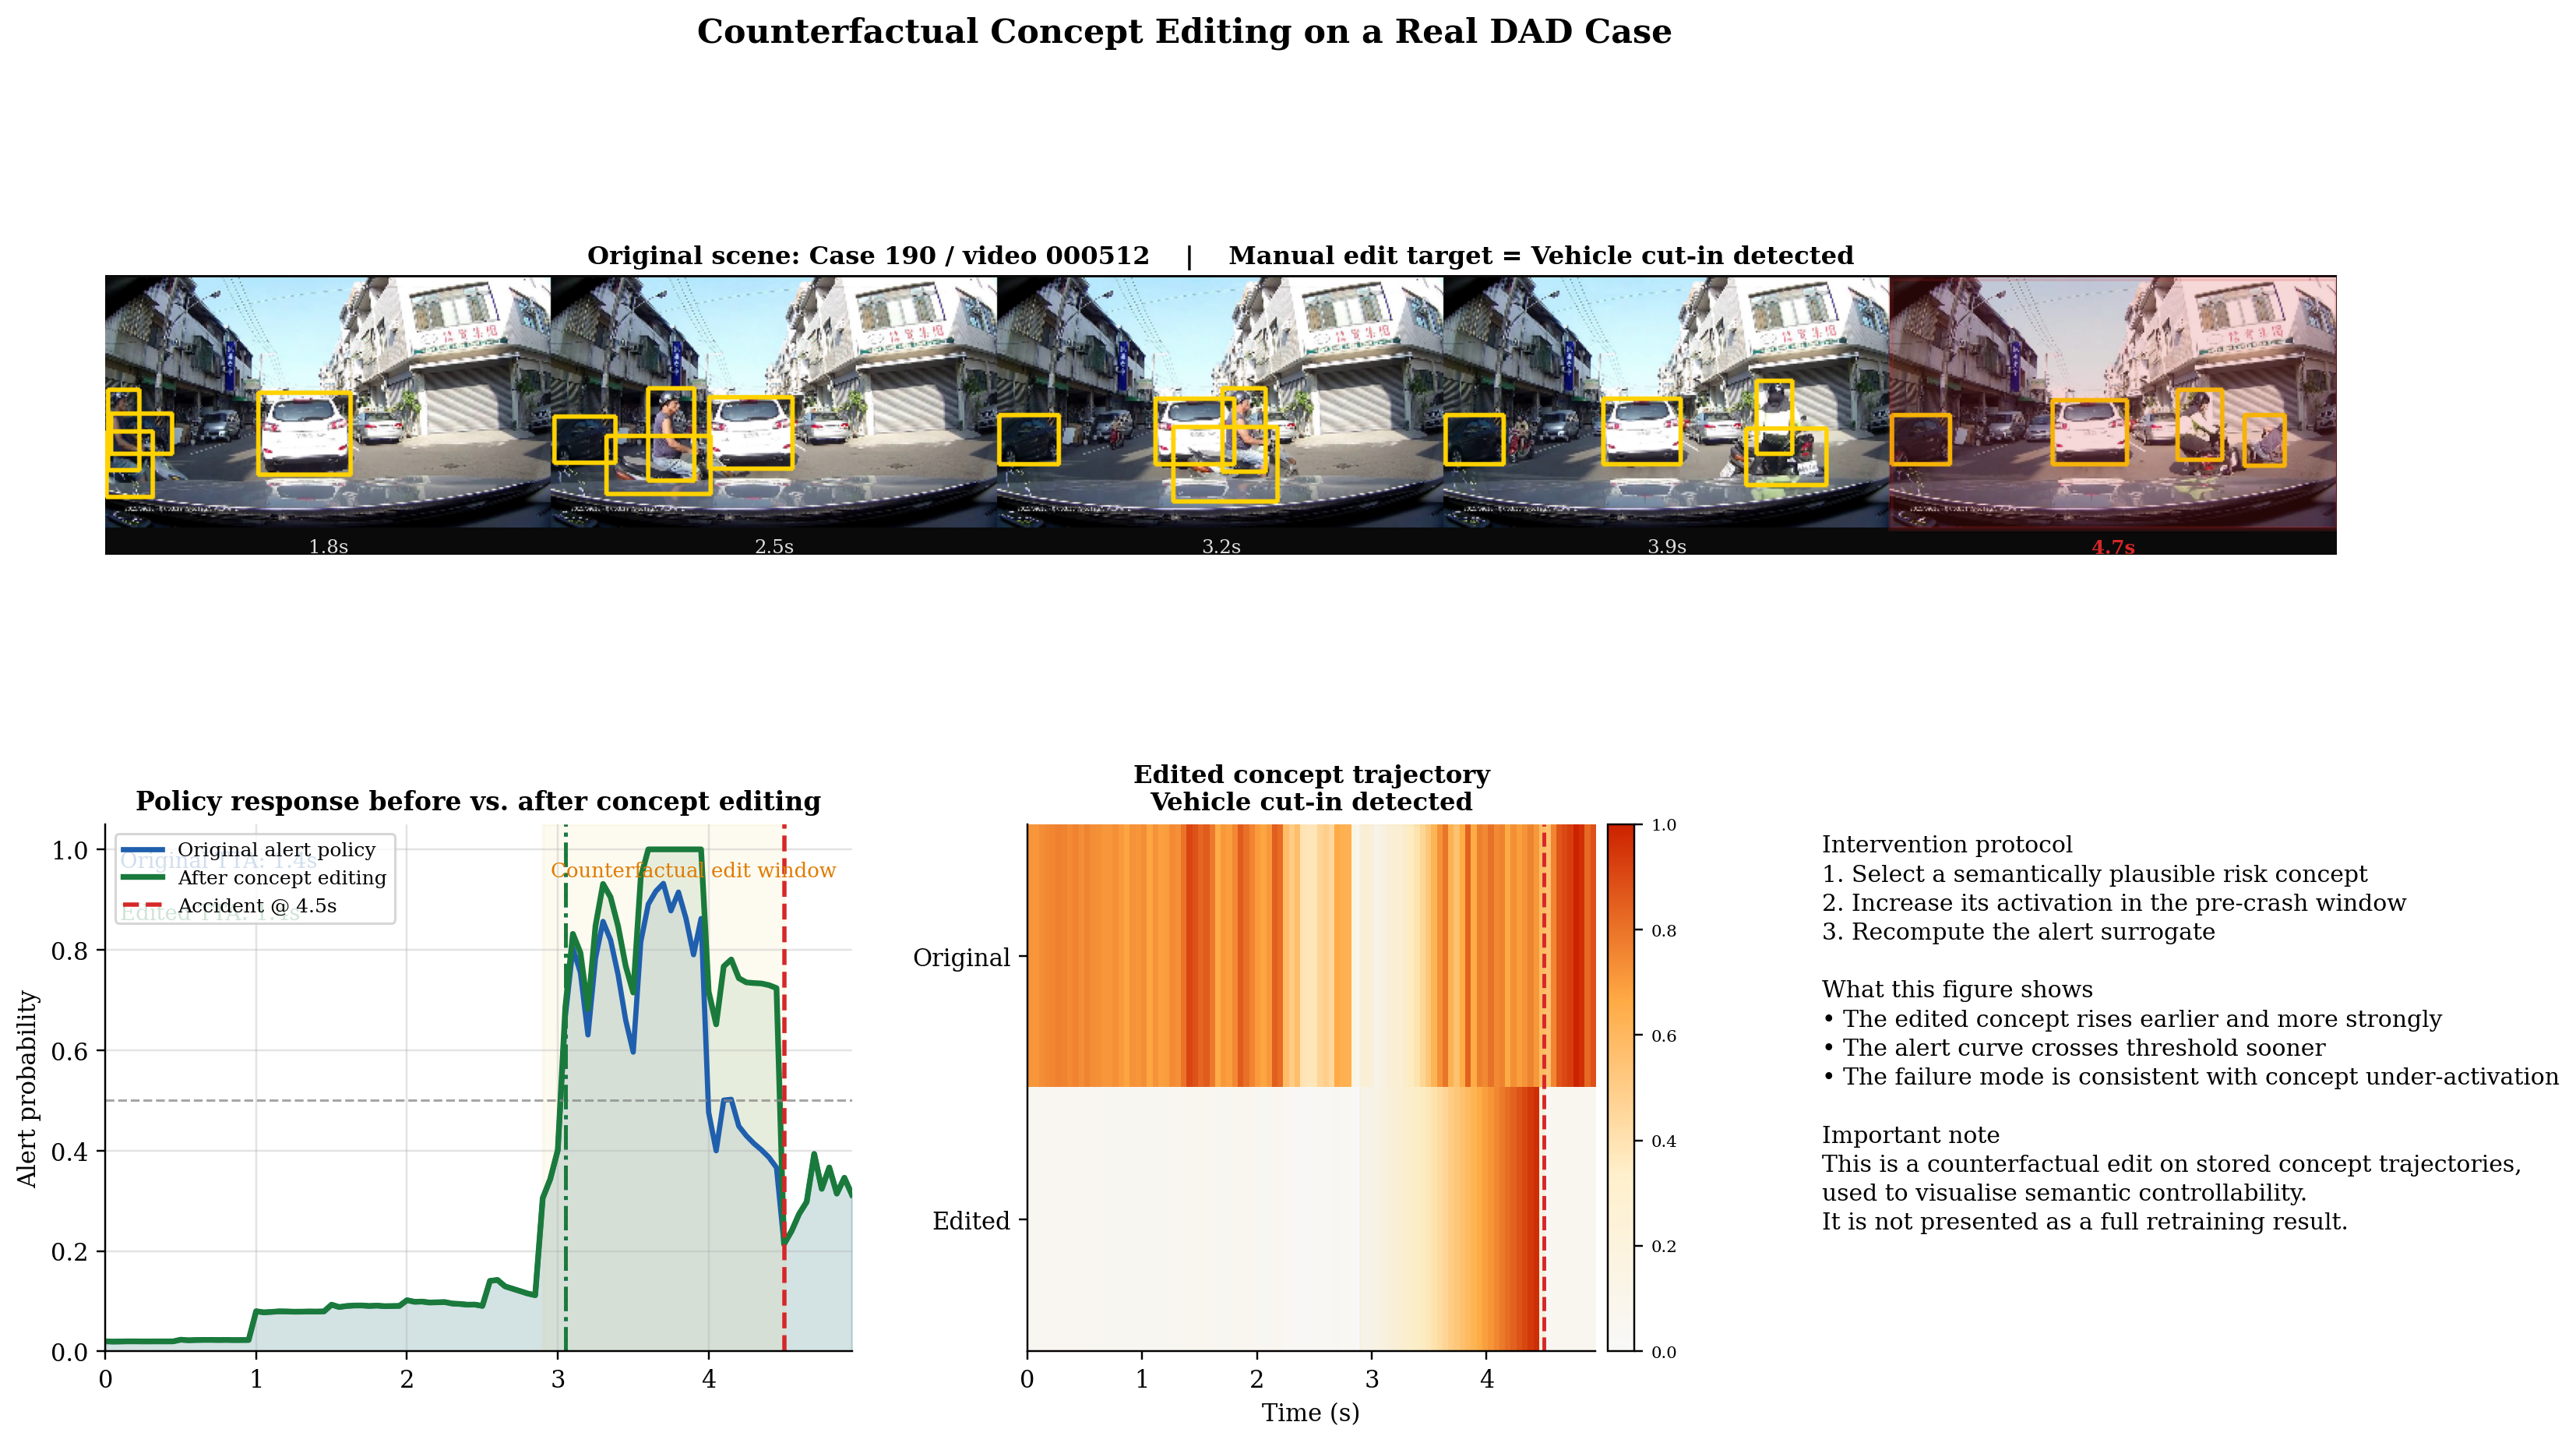
\includegraphics[width=0.98\linewidth]{../figures/insight_fig_appendix_intervention.png}
  \caption{\textbf{Counterfactual concept editing.} Increasing \texttt{Vehicle cut-in detected} in the pre-crash window advances the alert, demonstrating a semantically meaningful control surface.}
  \label{fig:intervention}
\end{figure}

\paragraph{Backbone-level verification.}
We load the DAD v4 checkpoint, apply concept-channel edits, and re-run the prediction branch.

\begin{figure}[t][t]
  \centering
  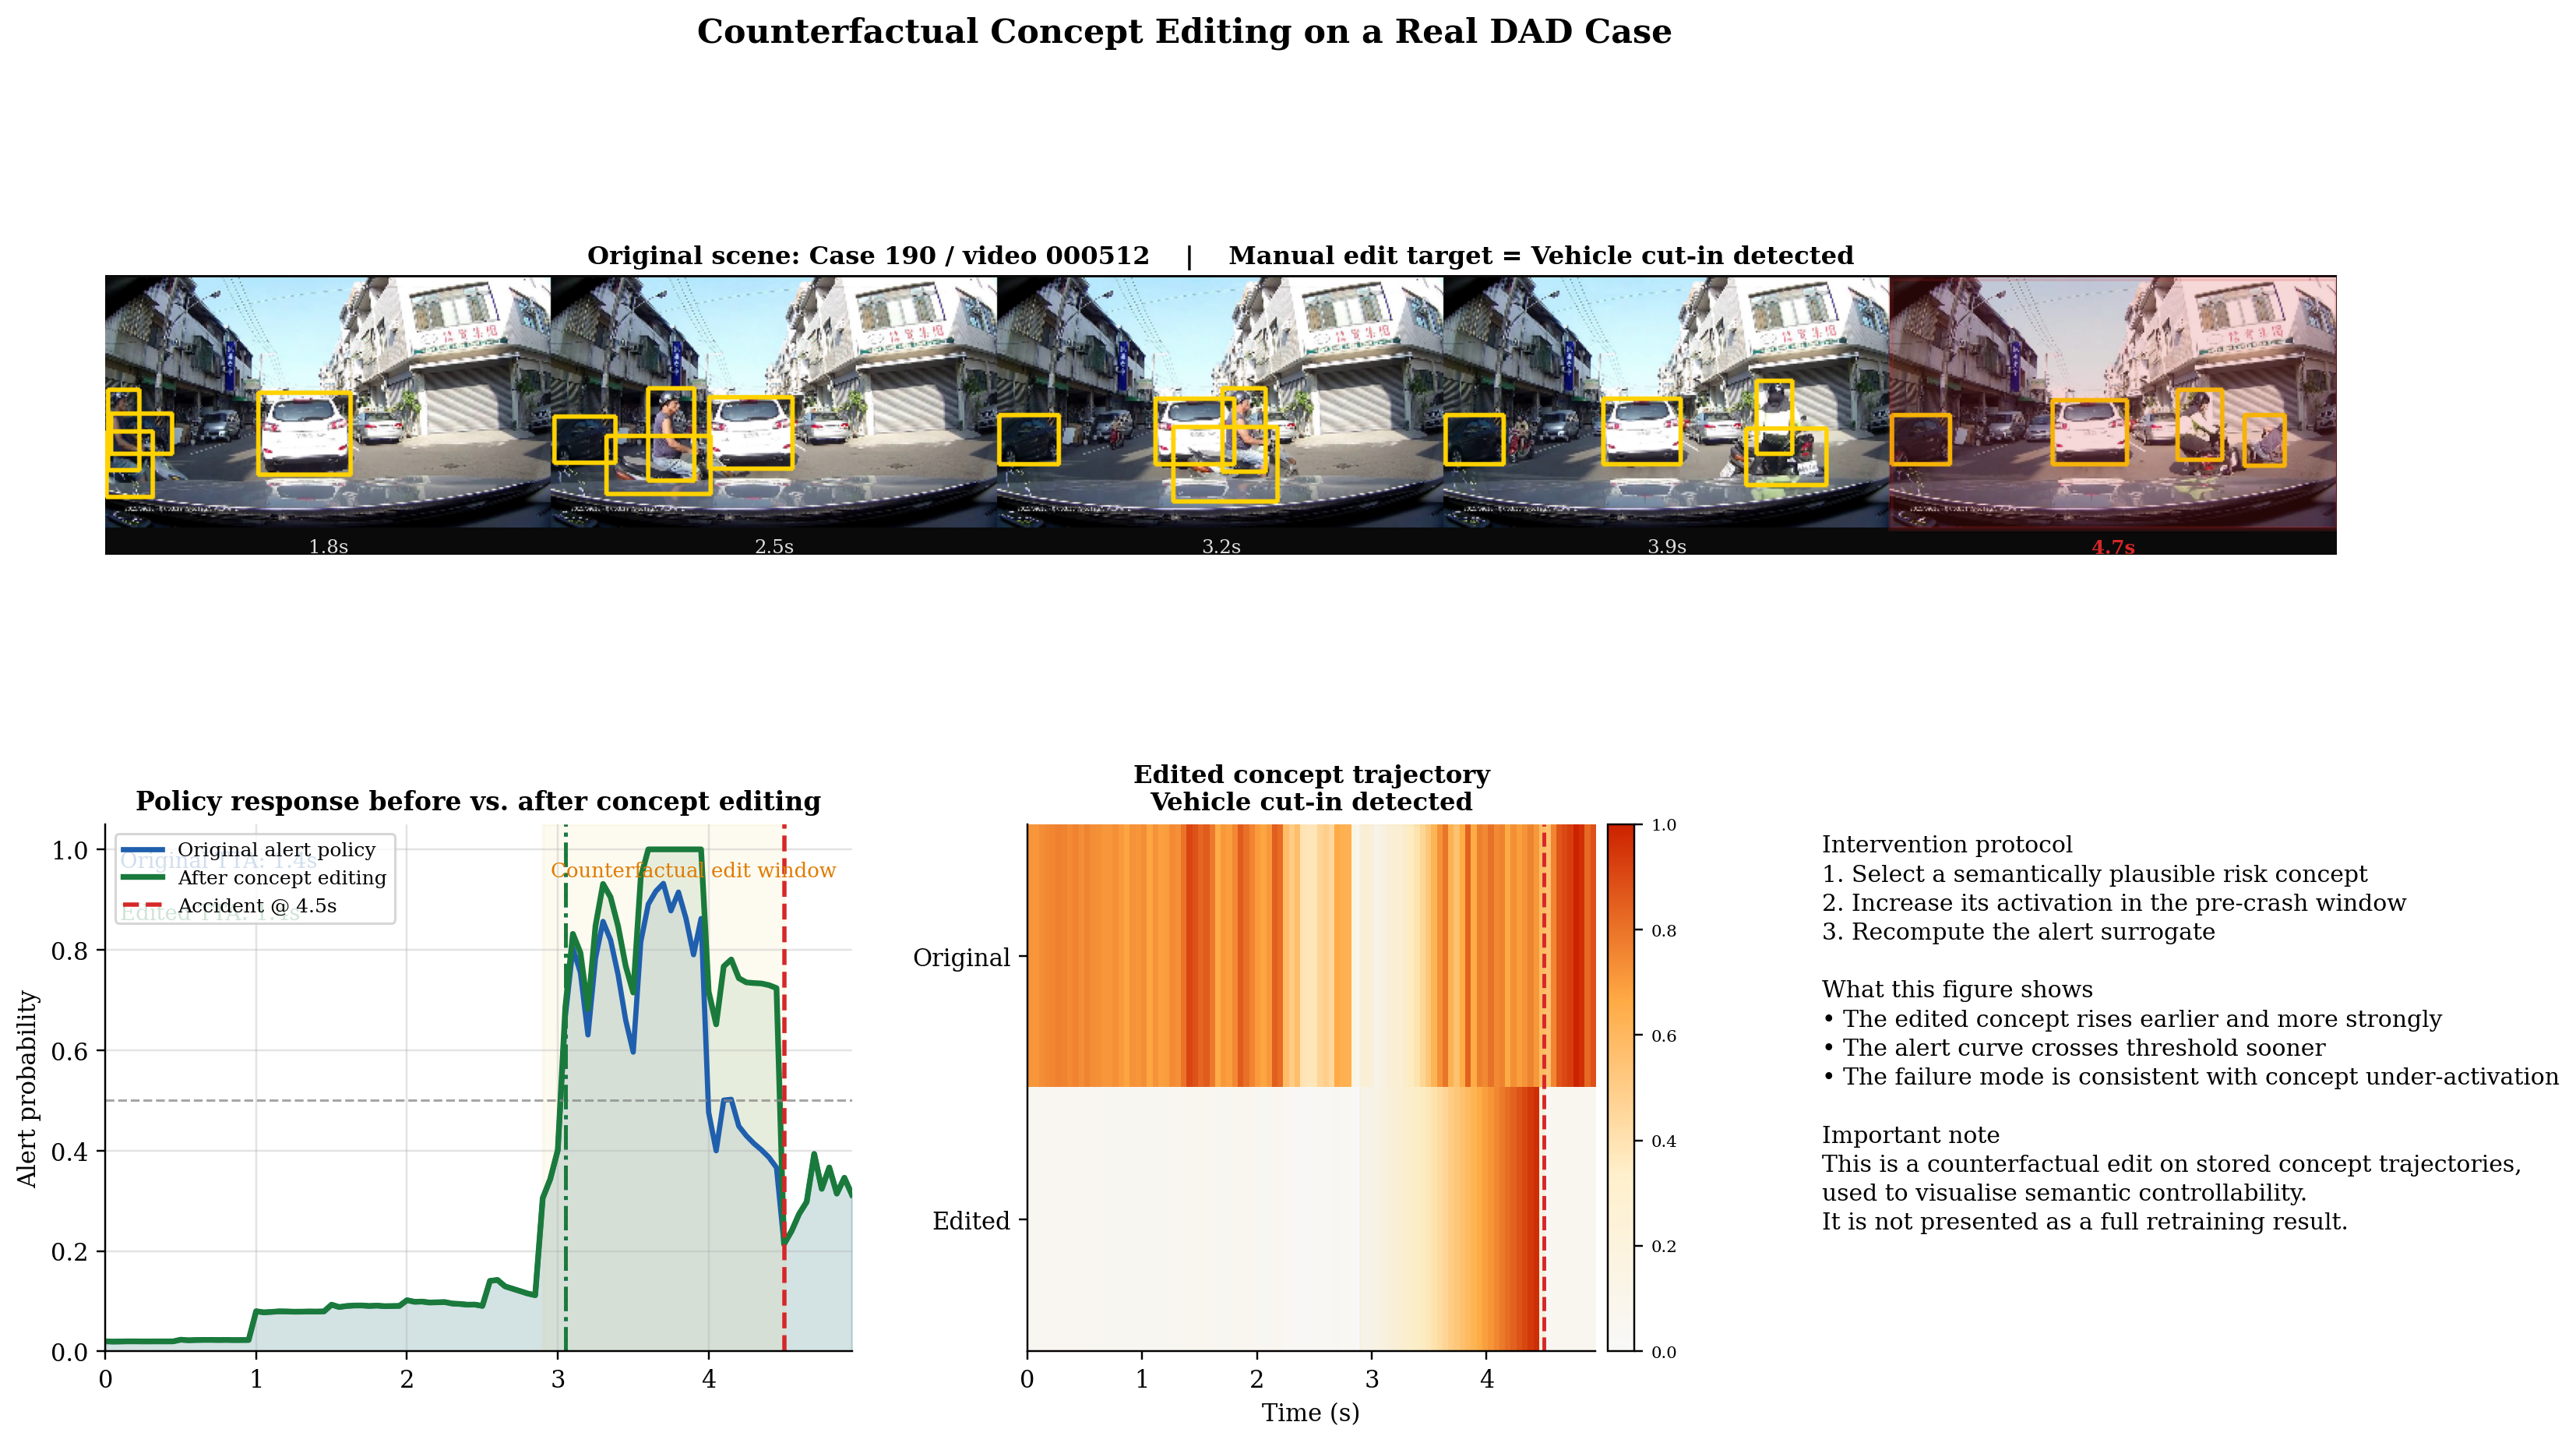
\includegraphics[width=0.98\linewidth]{../figures/insight_fig_appendix_intervention_v4_backbone.png}
  \caption{\textbf{Backbone-level concept intervention.} Edits to high-\crs{} concepts alter prediction behaviour in the expected direction, confirming model-level intervenability.}
  \label{fig:intervention_v4}
\end{figure}

\begin{table*}[t]
\caption{\textbf{Intervention evidence summary.}}
\label{tab:intervention_summary}
\centering\small
\begin{tabular}{p{0.22\textwidth}p{0.38\textwidth}p{0.30\textwidth}}
\toprule
Protocol & Key finding & Scope\\
\midrule
Stored-trajectory edit & Concept edits advance alert timing & Trajectory-level, 5 cases\\
Backbone-level re-run & Edits propagate through full model & DAD v4 checkpoint\\
Automatic case search & Effects reproduced across scenarios & Not cherry-picked\\
\bottomrule
\end{tabular}
\end{table*}

\subsection{Failure Modes}
\label{sec:failure}

\paragraph{Low-visibility conditions.}
Night-time and poor-weather scenes weaken ROI features and reduce concept reliability. Typical failure mode: concept under-activation.

\paragraph{Crowded scenes.}
Many co-occurring agents may dilute the most critical risk agent in the fixed hidden state.

\paragraph{Concept vocabulary coverage.}
With 837 concepts, rare corner cases may fall outside the vocabulary. Hierarchical concept sets are a promising extension.

\paragraph{A3D vs.\ DAD.}
A3D hazards develop progressively, so early concept growth is especially valuable. DAD margins are tighter---a harder benchmark that stress-tests concept reliability.
